\documentclass[twocolumn, a4paper,11pt]{article}%
\usepackage{graphicx}
\graphicspath{ {images/} }
\usepackage{cite}
\usepackage[utf8]{inputenc}
\usepackage[T1]{fontenc}
\usepackage{geometry}
\usepackage[font=scriptsize,labelfont=bf]{caption}
\usepackage{subcaption}
\def\BibTeX{{\rm B\kern-.05em{\sc i\kern-.025em b}\kern-.08em
		T\kern-.1667em\lower.7ex\hbox{E}\kern-.125emX}}

     % \textwidth 20cm
      %textheight 22cm
      %%%%%%parindent 10pt
      %\oddsidemargin 0.25cm
      %\evensidemargin 0.5cm
     \geometry{a4paper, 
     	total={170mm,257mm},
     left=20mm, 
     top=20mm,}
     
\usepackage{listings}
\usepackage{xcolor}
\lstset{%
	language=C++, %
	backgroundcolor=\color{black!5}, %
	basicstyle=\tiny, %
	}


\begin{document}

\thispagestyle{empty}
\onecolumn

\begin{center}

Vrije Universiteit Amsterdam

\vspace{15mm}


\includegraphics[height=28mm]{vu_griffioen.png}

\vspace{1.5cm}

{\Large Bachelor Thesis}

\vspace*{1.5cm}

\rule{.9\linewidth}{.6pt}\\[0.4cm]
{\huge \bfseries Implementation of the improved Peterson Kearns rollback algorithm\par}
{\huge \bfseries \par}\vspace{0.4cm}
\rule{.9\linewidth}{.6pt}\\[1.5cm]

\vspace*{2mm}

{\Large
\begin{tabular}{l}
{\bf Author:}	Robbert Alexander Rutte 	(2655858)
\end{tabular}
}

\vspace*{1.5cm}

\begin{tabular}{ll}
{\it 1st supervisor:}   & W.J.Fokkink \\
{\it 2nd reader:}       & ~~supervisor name
\end{tabular}

\vspace*{2cm}

\textit{A thesis submitted in fulfillment of the requirements for\\ the VU Bachelor of Science degree in Computer Science }

\vspace*{1cm}

\today\\[4cm] % Date

\end{center}


\newpage

\setlength{\columnsep}{.7cm}
\twocolumn

\begin{abstract}
	
\par In a distributed computer network it is important that the system is resilient and that the data integrity is maintained, furthermore it should be able to handle concurrent failures and  have a consistent state when ending execution. One of the protocols that satisfies these criteria is the Peterson-Kearns Rollback Recovery protocol. The algorithm is based on a vector-based clock to be able to establish a causal order of the messages. 
\par In this thesis the improved Peterson-Kearns Rollback Recovery protocol\cite{van2023optimistic} will be implemented and experimented with. It includes  a background study, discusses the limitations and challenges for the implementation of the protocol,  implements the protocol and measures its overhead and efficiency. The experimentation will include both the memory overhead, communications overhead and the run-time complexity of the implementation.
\par 
%after report the finding in small
	
\end{abstract}


\section{Introduction}
\par In the field of distributed computing, a complex system of processes that  participate to accomplish a shared goal, inter-process communication (IPC)  is indispensable asset. Yet as crucial as inter-process communication is, it also brings a surplus of complications and complexities that require thorough consideration and planning. From data consistency problems, ensure system resilience to minimizing communications overhead. 
\par The protocol discussed in this thesis aims to tackle the data consistency and  system resilience problems. The improved Peterson-Kearns Rollback recovery protocol is able to handle multiple concurrent failures without the program ending in an inconsistent state. In the next section the protocol will be described.

\subsection{Improved Peterson Kearns rollback algorithm}
\par The protocol provides data integrity and system resilience through the means of  of periodically checkpointing the IPC messages to stable storage. however even when operating in a FIFO channel environment  a failure of a process could result in an inconsistent state. For a message's send event could be lost to a failure if it is send causally after the last checkpoint. 
\par In the algorithm optimistic recovery is  considered, witch indicates that the checkpointing of the nodes is not synchronized. the rollback procedure handles the uncoordinated nodes reach a consistent state. It will do so by handling the \textit{lost messages}, messages where the receive event was lost in a failure at a crashed process or was rolled back to achieve a consistent state, and \textit{orphaned messages}, messages where the send event was lost in a failure at a crashed node or was rolled back. Once the process initiates the  restart or rollback procedure the execution is postponed and the messages that arrived are buffered to be handled once the process has restarted or rolled-back. 
\par The protocol relies on a vector based clock that is used to determine the causal order of the messages. To ensure the consistency of the system the Peterson-Kearns protocol relies on a logical vector clock to calculate witch events are causally after events that are lost in a failure.  each of the processes will maintain a clock vector and a failure vector  to ensure the the ability to uniquely identify failures. The failure vector ensures a consistent state when processes fail concurrently. An in-depth description of the protocol will be provided in Section II

\subsection{Context}
Inter-process Communication is a vital part of computer science and facilitates an operating system or a distributed system a way to let different processes communicate and cooperate to accomplish a task.  While IPC is inescapable to accommodate cooperation and communication between processes it also numerous problems such as reliability and fault tolerance. A system must be resilient enough to deal with failures to ensure consistency and reliability. The performance overhead must also be optimized since processes that use IPC incur a overhead in computational and memory resources. Furthermore IPC is also inherently more vulnerable to security threats, this must be managed to ensure the confidentiality and integrity of the data.  A system must also be synchronized  to avoid race conditions or a system must have ways to deal with race conditions. If a system uses shared memory across processes this must be well managed to ensure its correctness.
IPC is a well established in computer science. 

\subsection{Problem statement}
Distributed systems can always be affected by failures, like processes crashing, software errors or outside factors. All of these will be affecting the system consistency and correctness of the algorithm being executed. To prevent the failures from impacting the system implementing a rollback procedure is crucial. The rollback procedure will ensure that any event that is affected by a failure will be undone and forces the system to resume execution from a previously checkpointed consistent state. This will ensure the correctness and the consistency of the system.

\subsection{{Objectives}}
The objective of this thesis is to implement the improved Peterson-Kearns rollback protocol. The protocol should facilitate the system to:
\begin{enumerate}
	\item Enable its processes to notify others of a failure that occurred.
	\item Be able to respond to these failures.
	\item Rollback the events affected by the failure.
	\item Resume execution from a consistent state.
	\item Provide an efficient way to implement the procedure
	\item Minimize the communication  and performance overhead of normal execution.
\end{enumerate}

\subsubsection{Scope}
The scope of this thesis includes:
\begin{itemize}
	\item Implementing the improved Peterson-Kearns protocol.
	\item Testing the procedure under various scenarios to ensure the correctness of the implementation.
	\item Assess the performance, memory overhead and the communication overhead.
\end{itemize}
This Thesis will provide:
\begin{itemize}
	\item The implementation of the procedure with the source code and documentation.
	\item The test cases used to evaluate the correctness of the implementation.
	\item The measurement results and evaluation of the results.
	\item Indicate areas that could be optimized and enhanced based upon the measurements.
\end{itemize}

\subsubsection*{Constraints}
\begin{itemize}
	\item The rollback procedure is to designed to minimize the performance overhead, since this is an optimistic recovery algorithm, under normal operation of the implementation. 
	\item Minimize the memory overhead of the implementation. 
	\item Mimic the \textit{read()} and \textit{write()} c functions to facilitate easy usage of the implementation.
	\item The rollback procedure should maintain a consistent state.
\end{itemize}
\par In section 2  a study of the background of rollback algorithms and related work will  be done. Afterwards in section 3 the improved Peterson-Kearns protocol will be explained in detail, the design choices will be explained, the limitations of the implementation will be specified and the challenges of the implementation will be mentioned. In the fourth section the methodology will be described, the research goal and the implementation details will be provided.  The results of the experimental findings and analysis of these results will be done in the 5th section as well as an indication where more improvements could be made. The conclusion will be located at the 6th section.

\section{Background}
\par Rollback algorithms originate from the database field of computer science, they were first employed to ensure the consistency of a database system and to assure the atomicity and persistence of transactions when failures occur. The types of rollback algorithms that exist are categorized in two segments: \textit{Immediate rollback}, where the algorithm rolls back the affected events  immediately after detecting that a failure has occurred  and \textit{Deferred rollback}, where the algorithm defers the rollback of affected events  and handles them at a later time. 
\par \textit{Checkpointing} is the periodically saving of events to stable storage. Checkpointing is a central component in every rollback algorithm since when a failure occurs that makes a process crash, it must  be reinitialize with part of the memory otherwise to maintain a consistent state the algorithm would need to rollback all events. Therefore to be able to resume from some earlier consistent state checkpoints of the events that occur at all processes need to be saved to stable storage. Checkpoints frequently include the state of the system and previously generated events.
\par \textit{Logging} is another critical component of rollback algorithms. A log is kept of the send and receive events that are processed by the process. This log is used when a failure occurs at another process to undo the changes that were made by events that are affected by the failure and restore the state to a consistent state. Logging frequently includes the execution order of the events. 
\par \textit{Coordinated checkpoints} is where all processes of a system coordinate the checkpointing. In that case the algorithm synchronizes the checkpointing of its processes. They are often used of a way to maintain a consistent global state. This enables the protocol to rollback to a certain checkpoint with all its processes which will achieve a consistent state. No further  processing of the checkpointed messages will be necessary since they will not exist.
\par  Since the inception of rollback algorithms they have been applied in many fields other than that of database systems, like in distributed systems and operating systems. Rollback algorithms are vital in databases, operating systems, distributed systems and other fields to handle failures and preserve a consistent state.

\subsection{Related Work}
\par in this subsection we will explore existing rollback algorithms and classify them as immediate rollback or deferred rollback.

\subsubsection*{Immediate rollback}
\par An immediate rollback algorithm is a protocol that will apply changes to the system immediately in addition it will maintain a log file where the applied changes are stored. This often involves committing procedures for every event to ensure the consistency of the system. Once a failure occurs the rollback procedure will undo the changes to the system that have not been committed yet. The major advantage of this method is that the recovery process will not be an expensive procedure, thus this method is usually preferred when failures occur often in a system. Examples of the immediate rollback algorithms are:
\par \textit{Immediate update} described in Principles of Transaction Processing\cite{bernstein2009principles}.  Where an event is either committed when it executes or it is rolled back immediately. These commits are coordinated with other processes. Once a failure occurs the current event is rolled back to ensure a consistent state. 
\par \textit{Compensation-based recovery} as described in Sagas\cite{garcia1987sagas}. In this algorithm when an events affects the state of a system a compensation event is stored in memory. Once a failure occurs the compensation event is executed to revert the state of the system to a consistent state.

\subsubsection*{Deferred rollback}
\par A deferred rollback algorithm is a protocol that delays the commit procedure of events. This involves the storing of events in a log. Once the commit procedure is complete the changes to the system stored in the log will be applied. Once a failure occurs the rollback procedure will remove affected events in the log and these events will not be affecting the system.   The advantages of this method is that the I/O messages will be kept low since multiple events are committed at once, thus this method is usually used if failures will  only occur periodically. Examples of deferred rollback algorithms are:
\textit{Vector based rollback-recovery} in Rollback based on vector time\cite{peterson1993rollback}. This is the original algorithm that the improved Peterson-Kearns recovery-rollback\cite{van2023optimistic} protocol is based upon. In this algorithm causal order of events is provided by a logical vector clock.  Once a failure occurs other processes are notified via tokens and the affected events are rolled back to maintain a consistent state.
\par \textit{Distributed transaction processing} as described in Checkpointing and Rollback-Recovery for Distributed Systems\cite{koo1987checkpointing}.  In this algorithm a two-phase-commit procedure is used to facilitate the rollback.  In the two-phase-commit procedure all processes coordinate the checkpointing to ensure a consistent state.



\section{Framework}
In this section an in-depth overview of the implemented protocol will be given.  This will be a summary of the information given in the original Msc thesis of van Eck,C\cite{van2023optimistic}.
\subsection{Classifying events}
\par  In this subsection all events will be classified. An event is either a sent or a received message both classified as a send event and a receive event respectively. When these events are affected by a failure they will become either an orphan event or a childless event, these will be further classified into orphan-arrived, orphan-in-transit, childless-lost and childless-orphan events.

\subsubsection{Orphan event}
\begin{figure}[h]
	\centering
	\begin{subfigure}{8cm}
		\centering
		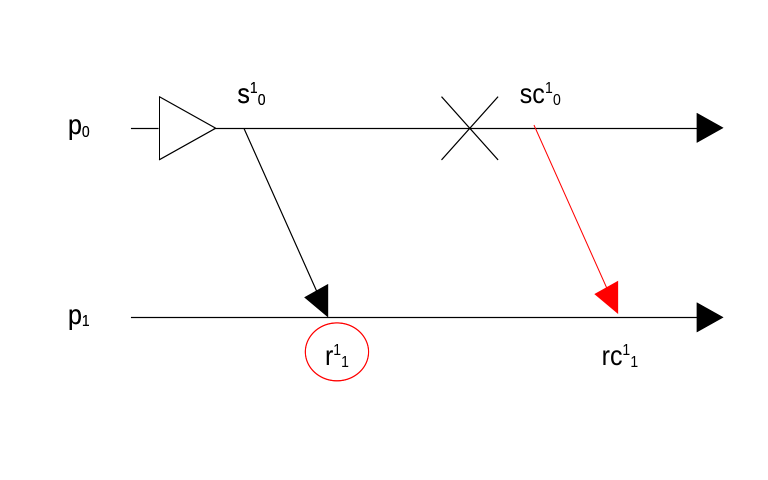
\includegraphics[width=8cm]{Orphan_arrived.png}
		\caption{Orphan-arrived}
		\label{fig:orphan_arrived}
	\end{subfigure}
	\begin{subfigure}{8cm}
		\centering
		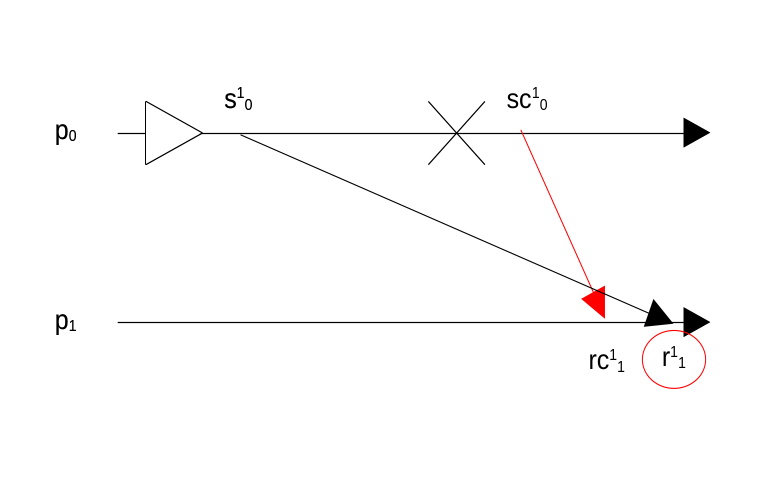
\includegraphics[width=8cm]{Orphan_in_transit.png}
		\caption{Orphan-in-transit}
		\label{fig:orphan_transit}
	\end{subfigure}
	\caption{Orphan events}
\end{figure}
\par An \textit{orphan event} is created when the send event of a receive event is lost in a failure, this lost send event will be causally after the last checkpoint at the failed process. 
\begin{itemize}
	\item \textbf{Orphan-arrived}: The receive event is causally before the rollback is performed, and is thus before the control message signaling a failure has arrived. Event \(r^{1}_{1}\) in figure   \ref{fig:orphan_arrived} becomes an orphan-arrived event after the failure at \(p_{0}\).
	\item \textbf{Orphan-in-transit}: The receive event is causally after the rollback has been performed, and is thus after the control message signaling a failure has arrived. Event \(r^{1}_{1}\) in figure \ref{fig:orphan_transit} is a orphan-in-transit event.
\end{itemize}

\subsubsection{Childless event}
\begin{figure}[h]
	\centering
	\begin{subfigure}{8cm}
		\centering
		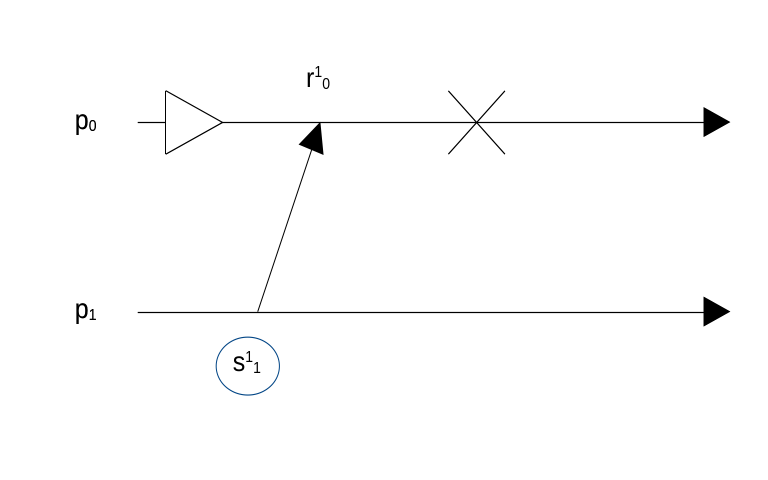
\includegraphics[width=8cm]{Childless_lost.png}
		\caption{Childless-lost}
		\label{fig:childless_lost}
	\end{subfigure}
	\begin{subfigure}{8cm}
		\centering
		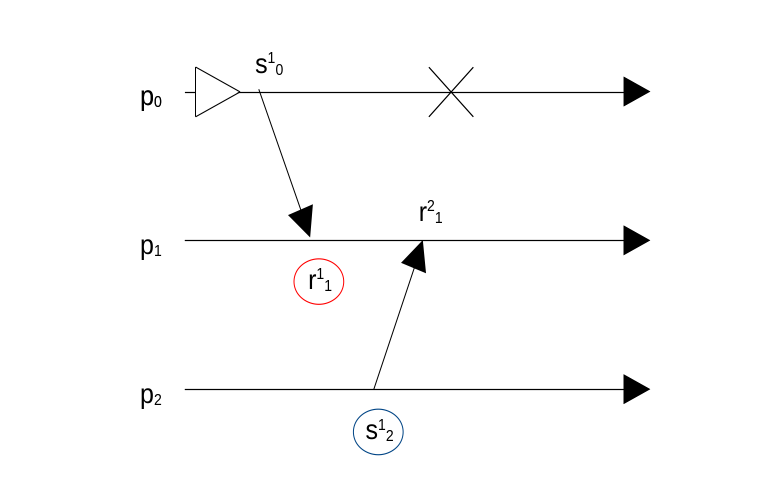
\includegraphics[width=8cm]{Childless_orphan.png}
		\caption{Childless-orphan}
		\label{fig:childless_orphan}
	\end{subfigure}
	\caption{Orphan events}
\end{figure}
\par A \textit{childless event} is created when the receive event of a send event is lost in a failure,  this lost receive event will either be itself lost in the failure or will be lost in the rollback of another process. 
\begin{itemize}
	\item \textbf{Childless-lost}: The receive event that is lost is causally after the last checkpoint at the failed process, and is thus itself lost in the failure. Event \(s^{1}_{1}\) in figure \ref{fig:childless_lost} becomes a childless-lost when the failure at \(p_{0}\) occurs.
	\item \textbf{Childless-orphan}: The receive event that is lost is causally after an orphaned event at another process, and is thus lost in the rollback procedure at the other process. Event \(s^{1}_{2}\) in figure \ref{fig:childless_orphan} becomes a childless-orphan after the failure at \(p_{0}\) occurs.
\end{itemize}


\subsection{Algorithm Overview}
\par The improved Peterson-Kearns Rollback recovery protocol\cite{van2023optimistic} has several procedures that are needed for the protocol to function correctly. The protocol employs vector clocks to determine what events are affected by a failure. Each process keeps track of 2 vector clocks, a clock for keeping track of both casual order of the events, the time vector, and the number of times a process has crashed, the failure vector.  Both of these clocks will be sent along with a message to inform other processes of the current state of the vector-clock at the sending process. All events will be stored in volatile memory along with its accompanying vector clocks. 

\subsubsection{Time Vectors}
\par Each process has an associated time vector. The time vector \(T= T^{0},...,T^{n-1}\) gets updated whenever an event \(e_{i}\) occurs where \(n\) is the  number of processes and \(i\) is the process id where the event occurred.  The \(T'\) notation is the time vector before the event \(e_{i}\) occurred.
\begin{itemize}
	\item When \(e_{i}\) is a send event then the time vector \(T\) of a process gets updated to \(T^{i} =  T'^{i} + 1\).
	\item When \(e_{i}\) is a receive event  the time vector \(T\) of a process gets updated to \(T^{j} = max(T'^{j}, e_{i}.T^{j})\) where \(j \neq i\) and \(T^{i} = T'^{i} + 1\)
\end{itemize}

\subsubsection{Failure vectors}
\par Each process has an associated failure vector, the failure vector  \(F = F^{0},...,F^{n-1}\) gets updated when a failure occurs in a process or the process get notified of a failure at another process. 
\par In the case of the failure failure happening at the current process will perform the restart procedure, and therein the failure vector gets updated to \(F^{i} = F'^{i} +1\) where \(i\) is the id of the current process, afterwards the process sends control messages to all other processes to notify them of its failure. This control message includes:
\begin{itemize}
	\item \(id\): The process ID of the failed process.
	\item \(n\): The failure number, indicating the amount of failures that occurred in total at the failed process.
	\item \(T_{i}^{i}\): The restart time, indicating the \(T^{i}\) at the moment of restart at the failed process.
	\item \(arrived\): The set of \((T^{j}, F)\)  of the messages received by the failed process that were sent by the process \(p_{j}\) receiving the control message.
\end{itemize}
In the case that the failure did not occur at the current process, then the current process will be notified of the failure by receiving a control message. When the control message is received the process will perform the rollback procedure, and therein the failure vector will be updated to \(F^{j} = n\) where \(n\) is the value received in the control message for the failure number and \(j\) is the process ID of the failed process.

\subsubsection{Checkpoint procedure}
During a checkpoint procedure all information needed to restore the process to a stable state are stored in stable storage. The information to be saved in storage is as follows:
\begin{itemize}
	\item \textit{state} : the state of a process.
	\item \textit{T}: The time vector of the process at the moment the checkpoint occurs.
	\item \textit{log}: The log where the events that occurred at the process are stored.
\end{itemize} 
During a checkpoint procedure no other event can occur.

\subsubsection{Restart procedure}
\par After a failure at a process it will need to restart from the last checkpoint . The operations needed to perform the restart successfully are:
\begin{enumerate}
	\item The failure vector is updated to \(F^{i} = F'^{i} +1\) where \(i\) is the ID of the process where the failure occurred.
	\item The process will be restored to the latest checkpoint.
	\item Send control messages to the other processes.
\end{enumerate}
During a restart procedure no other events can occur.

\subsubsection{Rollback Procedure}
\par After a control message is received at a process it will need to perform a rollback to achieve a global consistent state. The operations needed to perform the rollback successfully are:
\begin{enumerate}
	\item The failure vector is updated to \(F^{i} = F'^{i}  + 1\) where \(i\) is the ID of the process where the failure occurred.
	\item If some event is orphaned at the process that received the control message, then the state is returned to the last checkpoint that does not include orphaned events. All events after this checkpoint that are not orphaned will be replayed.
	\item Any receive events that have been orphaned but have a corresponding send event that was not orphaned will have their receive event replayed.
	\item All messages that this process sent to the process where the failure occurred with a non orphaned send event that did not arrive will be re-transmitted.
	\item A new checkpoint will be created.
\end{enumerate}
During the rollback procedure no other events can occur.

\subsection{Limitations}
\par The limitations of this algorithm are that the maximum number of messages that can be sent by one process will be the upper-limit of the integers used in the time vector, this could be mitigated by allowing the time vector values to roll over back to zero in some way but this would require more logic to accommodate for this.  
\par Another limit of this algorithm would be that when the amount of events stored by a process becomes large and a failure occurs at that process it will need to sent a large set of messages that have arrived at that process.  This could be mitigated by occasionally checking what messages have been checkpointed by all processes and then committing these events.  After the set of arrived messages will not be needing messages in it that have been committed. This will be explained more in-depth.
\par If a task needs to be completed that will generate a large amount of event the volatile memory of a process could reach the allowed limit fast. to mitigate this some events could be removed if they have been committed and will not be needed for re-transmission. This would shrink the volatile memory needed for continuous operation. This will be explained more in-depth.

\subsubsection{Commit procedure}
When a commit procedure is initiated by a process commit messages will be sent between processes. A committed event will be stored in a separate file in stable storage. These messages will be as follows:
\begin{enumerate}
	\item the process initiating the commit procedure will signal all other processes.
	\item When this signal is received at a process it will send the initiating process the \(T^{i}\)  of its last \textit{checkpoint} where \(i\) is the process ID.
	\item After all of the aforementioned messages have been received the initiating process will construct a minimal checkpointed time vector from these values with its \(T^{i}\)  of its last \textit{checkpoint}.
	\item All events that have a time vector that is \(\leq\) the minimal checkpointed time vector can be committed.
	\item  The initiating process will send this minimal checkpointed time vector to the other processes. Along with the list of committed receive events that have been sent by the recipient of this message, this is needed for the removal of send events.
	\item All processes will now be able to commit events, if the process is not the initiator of the commit procedure it will send all other processes a list of of committed receive events that have been sent by the recipient of the message, this is needed for the removal of send events.	
\end{enumerate}
in between commit messages other event can occur.

\subsubsection{Remove procedure}
\par After all of the other processes have sent the list of committed receive events to a process it can perform the remove procedure. \textit{NextCk(\(e\))} is the checkpoint after the one event \textit{\(e\)} is stored in. the events that can be removed are as follows:
\begin{itemize}
	\item \textit{Messages stored in volatile storage}: all events \textit{\(e\)} that have \textit{NextCk(\(e\))} \(\leq\) the minimal checkpointing time vector  can be removed. if \textit{e} is a sent event its corresponding receive event needs to be contained in the set of committed messages received during the commit procedure.
	\item \textit{Checkpoints stored in stable storage}: All checkpoints \textit{\(ck_{i}\)} can be removed if \textit{NextCk(\(ck_{i}\)} \(\leq\) the minimal checkpointing time vector.
	\item \textit{Failures stored in stable storage }: these can only be removed when FIFO channels are used.
\end{itemize}

\subsection{Design Choices}
Since one of the requirements of the implementation is that operation without failures occurring should have a small overhead the implementation will be written in C++. In addition to that to ensure fast operation of vector logic the vector package from the C++ standard library was used. To ensure low overhead on the sending and receiving procedures no loops were used in this part of the implementation. The functions to send and receive messages are modeled after the C write and read functions to facilitate simple usage of the implementation.
\par An implementation will be made for the base protocol without the commit and remove procedures, as well as a version with the commit and remove procedures to test them against each other for a difference in performance. 

\section{Methodology}

\subsection{Research Goal}
\par The goal of the experimental setup is that the implementation will be tested on performance.  The performance tests that will include the testing performance of both the implementation with and without the commit and remove procedure. For both of these the performance of the sending and receiving of messages will be measured. The performance of the Restart and Rollback procedure will also be measured. The performance of the rollback procedure will also be measured when dealing with concurrent failures from another process. Afterwards the measurements of both of the implementations will be compared.

\subsection{Implementation Details}
\par The implementation of the improved Peterson-Kearns rollback recovery protocol is written in C++ version 20.
\subsubsection*{State class}
The State class contains all components needed to maintain a consistent state. the main components of the class are the id of the process, the number of messages in volatile storage, the event log containing the message events, time vector,  failure vector, the file descriptors of all other processes(these will be used to resend lost messages), checkpoints and checkpoint time vectors, a set arrived messages and a set of arrived control messages. The version of the class where committing and removing messages is possible the State class also includes a vector to track if the commit or remove procedures can be executed, a set of committed messages, a set of committed receive events form the other processes and a minimal time vector to calculate the messages that can be committed and removed. The most important methods of the State class are listed below.
\par Public methods:
\begin{itemize}
	\item \textbf{State:}
	Initializes the class. If the initialization is executed with the restart boolean set to true it will execute the restart operation and sent controll messages to other processes.
	\item \textbf{checkpoint:}
	Performs a checkpointing procedure .
	\item \textbf{send\_msg:}
	Sends a message and increments the time vector. This will only send messages of type MSG
	\item \textbf{recv\_msg:}
	Receives all message types and handles them accordingly, it will receive normal messages that increments the time vector, it will receive control messages and initiate the rollback procedure, it will receive all commit messages and process them accordingly and it will receive void messages which will not affect the state of the process and will only be passed through to the caller of recv\_msg. The method uses c function read to read from its read file descriptor.
	\item \textbf{send\_ctrl:}
	Sends a control message to all other processes to indicate a failure has occurred. The methods uses  the c function write to write to the  file descriptor of other processes.
	\item \textbf{signal\_commit:}
	Signals to all other processes to start the commit procedure.
	\item \textbf{update\_fd:}
	Updates the file descriptors of a process.
\end{itemize}
The public methods also include methods to retrieve the stored event log.

\par In addition to these public methods the class has several private methods that are used by the class to operate. The most important private methods of the State class are listed below:
\par Private methods:
\begin{itemize}
	\item \textbf{check\_duplicate:}
	Checks if a received message is a duplicate .
	\item \textbf{check\_duplicate\_ctrl:}
	Checks if a recieved control message is duplicate.
	\item \textbf{check\_duplicate\_commit:}
	Checks if a message has already been committed.
	\item \textbf{check\_orphaned:}
	Checks if a received message is orphaned.
	\item \textbf{rem\_log\_entries:}
	Removes log entries from from the event log.
	\item \textbf{rem\_checkpoints:}
	Removes checkpoints.
	\item \textbf{store\_msg:}
	Stores a message in the event log.
	\item \textbf{commit\_msgs:}
	Commits the indicated messages.
	\item \textbf{rollback:}
	Performs the rollback procedure. This procedure could resend messages that were lost in the failure to the failed process.
	\item \textbf{send\_commit:}
	Sends its own the time vector value to the process that initiated the commit procedure.
	\item \textbf{commit :}
	Performs the commit procedure and sends the committed receive events to all other processes.
	\item \textbf{remove\_data:}
	Performs the remove procedure.
\end{itemize} 
The private methods also include serialization methods and methods to calculate various pointers and indices. 
The \textbf{send\_void} function is included in the  namespace Pet\_kea. It send a message to a process that does not increment the time vector and is not stored in the event log.
\par the class is able to send the types of messages listed below:
\begin{itemize}
	\item \textbf{MSG:} This is a message that will be processed by the protocol, it increments the time vector of the process. It includes the time vector and failure vectors at the time of sending, the ID of the sending process and the message size in bytes.
	\item \textbf{CTRL:} This is the message that will be send if a failure has occurred, it will increment the failure vector of the process receiving it. It includes the failure log entry, the ID of the sending process, the amount of messages the sending process has received from the receiving process of the control message and the time vector value and failure vector of these messages. this message can only be sent after a process has restarted.
	\item \textbf{VOID:} This is the message that will not impact either the time vector or the failure vector and will be passed trough to the caller of the \textbf{recv\_msg} method. And thus not affecting the state of the protocol. This would be used when a message has to be sent between processes that can not alter the state.
	\item \textbf{COMM1:} This is the message that will be sent to initiate the commit procedure
	\item \textbf{COMM2:} This message will contain the its time vector value of its latest checkpoint.
	\item \textbf{COMM3:} This message will contain the combined time vector values of the latest checkpoints of all the processes. These will be used to determine which events can be committed and removed.It also contains the receive events from messages send by the receiver of this COMM message that have been committed by the sender of the COMM message in addition to this the amount of these receive events in the message. This message will be sent by the initiator of the commit procedure only. 
	\item \textbf{COMM4:} This message will contain the receive events from messages send by the receiver of this COMM message that have been committed by the sender of the COMM message in addition to this the amount of these receive events in the message. This message will be sent by the non-initiators of the commit procedure only. 
\end{itemize}
\par The event log consists of an array of structs that contain the send and receive events that are stored, message size, the ID of the message that send the message, the time vector at the moment of sending, the time vector at the moment of receiving and the failure vector at the moment of sending. it also contains the index of the next checkpoint and a boolean indicating if the messages is a send or a receive event.

\subsection{Experimental Setup}
The experimental setup that was used to measure the overhead cost of the implementation operates as follows:
\par A parent process  creates pipes for its child processes to communicate and then forks them. The child processes will then randomly send each other messages using the State class. The parent process is then able to interrupt one of its children by sending them a SIGINT interrupt. This interrupt is then caught by the child process which will then complete its current select loop and will then exit. After the child has exited the parent will restart the process by forking it again.  A process will transmit its new file descriptors over UNIX domain sockets.
The child processes will use a select loop to deal with the incoming messages of the other processes.
\par The experiments will be run on a dell XPS 13 using a intel i7-8565U CPU running at 1.80GHz, the operating system used was ArchLinux 2024.05.01 release with the included kernel version 6.8.8.  Both the implementation of the protocol and the experimental framework is written in C++ version 20. 
\par The measurements are taken using the chrono::high\_resolution\_clock from time.h.  The measurements of the overhead cost for sending and receiving and checkpointing are taken by only measuring how long it took to complete the \textbf{send\_msg}, \textbf{recv\_msg} and \textbf{checkpoint} methods. For the restart time cost measurements are taken by measuring the time it took for the class to be initialized and transmit all control messages and thus resume normal execution using increasing number of messages stored in stable storage. For the rollback time cost measurements is the time it takes from the moment the process receives the control message until it has handled the rollback procedure and resumed normal operation, each subsequent time using increasing number of messages stored in its event log to determine what effect this has on the rollback procedure.
The communication overhead and stable storage memory overhead is calculated using the serialized size of the message and event log. The RAM memory overhead is calculated by the used memory space by the event log struct and the size of the accompanying vectors.
The measurements are saved in a CSV file to be able to analyses the results more easily. 
\par In addition to the performance test a correctness test will be performed, various scenarios will be checked to indicate the correctness of the implementation. 


\section{Results and Analysis}
\subsubsection{Memory overhead}
\par The implementation of the improved Peterson-Kearns protocol both for storing messages in stable storage and in communication utilizes serialized data. The overhead for storing messages in stable storage:\[3*sizeof(int) + 3*sizeof(int)*n\ bytes\]the communications overhead:\[ 3*sizeof(int) + 2*sizeof(int)*n\ bytes\]and the overhead for storing messages in random access memory: \[96+3*sizeof(int)*n\ bytes\] where \[n = number\ of\ processes\] 
This shows that when this implementation is used by a large amount of processes that the memory overhead will increase substantially. This overhead could be diminished if an int16\_t would be used to store the time and failure vectors, however the downside to this would be that the implementation would be able to handle less messages.

\subsection{Experimental Findings}
\subsubsection{Sending performance}
\begin{figure}[h]
	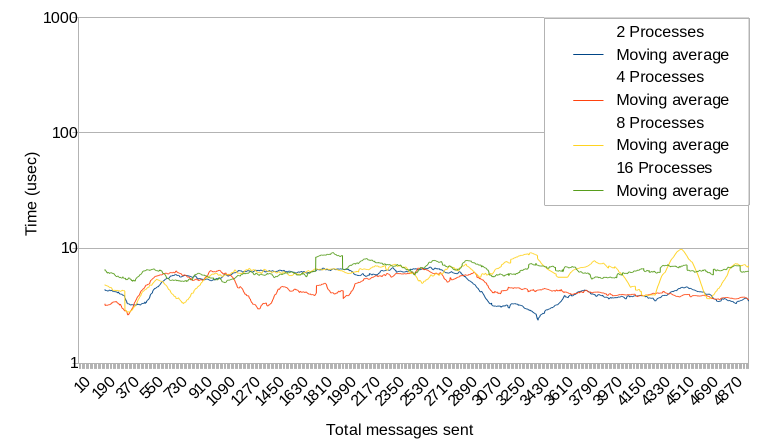
\includegraphics[width=8cm]{send_timing_commit_ma_new.png}
	\caption{Sending cost for one message : commit procedure (200 MA)}
	\label{fig:comm_send}
\end{figure}
\begin{figure}[h]
	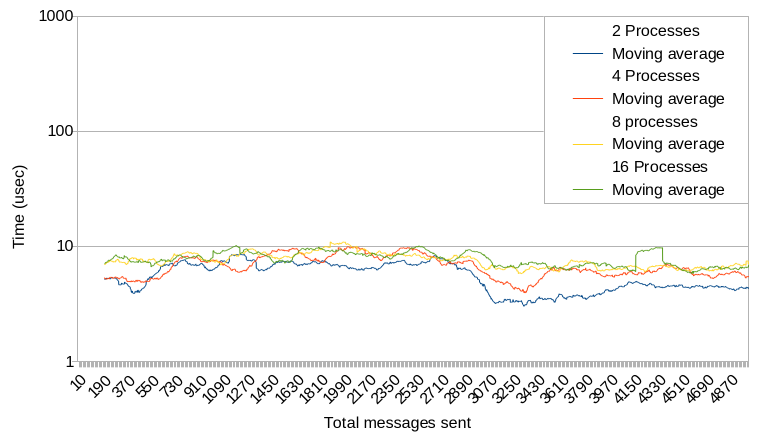
\includegraphics[width=8cm]{send_timing_nocommit_ma_new.png}
	\caption{Sending cost for one message (200 MA)}
	\label{fig:nocomm_send}
\end{figure}\noindent
The two figures \ref{fig:comm_send} , \ref{fig:nocomm_send} show the 200 moving average of time cost of sending a message. The sending cost is tested using different amounts of processes communicating. In the first figure the processes were committing and removing events as well as checkpointing the events, in the second figure the processes were only checkpointing the events. This shows that the sending performance is not affected by the increase in processes communicating. It also shows that there is not a big difference in sending cost between weather the messages will be committed or not, however this is to be expected since the operations used for sending a message do not change between the two versions of the protocol.

\subsubsection{Receiving performance}
\begin{figure}[h]
	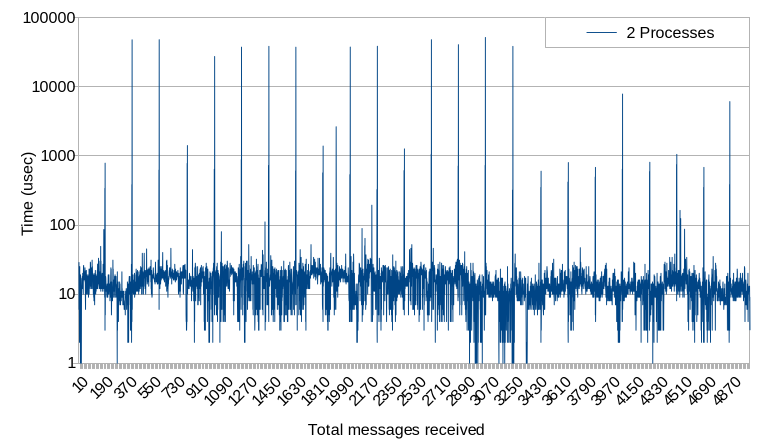
\includegraphics[width=8cm]{recv_timing_commit_2_processes_new.png}
	\caption{Receiving cost for one message : commit procedure}
	\label{fig:comm_recv}
\end{figure}
\begin{figure}[h]
	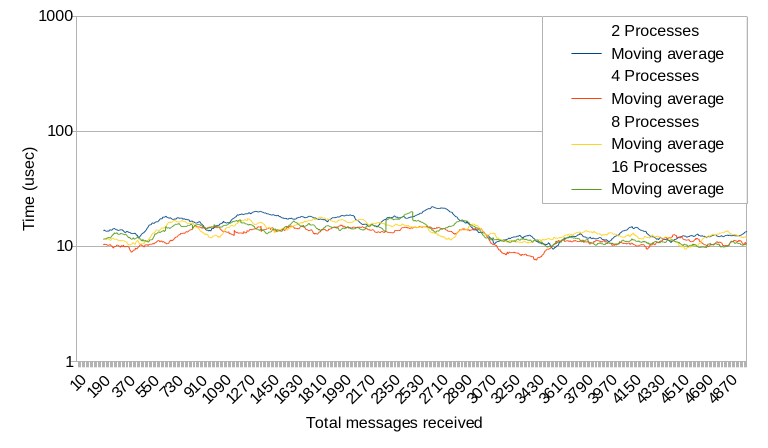
\includegraphics[width=8cm]{recv_timing_nocommit_ma_new.png}
	\caption{Receiving cost for one message (200MA)}
	\label{fig:nocomm_recv}
\end{figure}\noindent
The two figures \ref{fig:comm_recv}, \ref{fig:nocomm_recv} above show the receiving cost of receiving a message. The receiving cost is tested using different amounts of processes communicating. The first figure shows the performance while the processes are committing and removing events. for clarity only the plot for 2 communicating processes is shown. This shows that there are numerous spikes in the time cost if we look at the second figure we can see why this occurs. In the second figure a 200 moving average is used. Here we can see that we do not have such spikes in time cost and can thus conclude that the committing and removing events is a costly procedure. we can also see that the receiving performance is not affected by the increase in processes communicating.

\subsubsection{Restart performance}
\begin{figure}[h]
	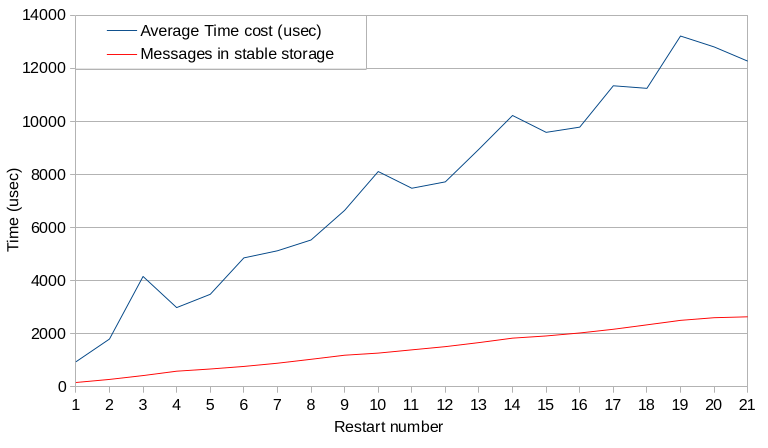
\includegraphics[width=8cm]{restart_timing_average_rode_lijn_new.png}
	\caption{Average restart cost}
	\label{fig:average_restart}
\end{figure}\noindent
The figure \ref{fig:average_restart} above shows the time cost of the restart procedure. The blue line shows the time it took from the moment the process called the constructor of the State class until normal operation was resumed, the red line the amount of messages in stable memory that where stored by the process performing the restart. This shows that the time cost of the restart procedure is proportionate to the amount of messages that are stored in stable storage, furthermore it shows that restarting is relatively a cheap procedure. 

\subsubsection{Rollback performance}
\begin{figure}[h]
	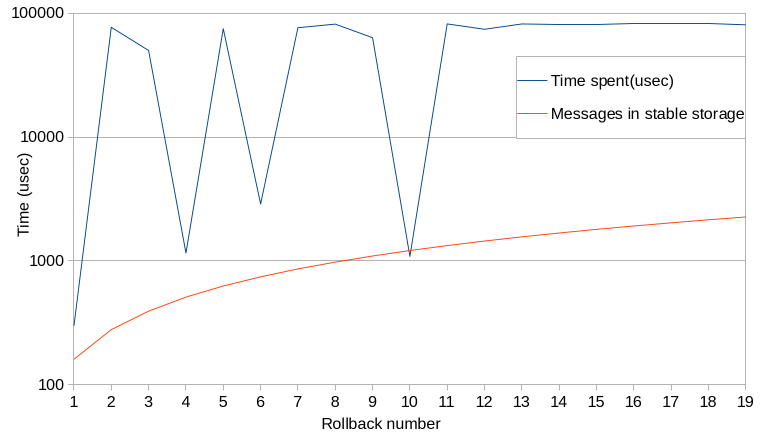
\includegraphics[width=8cm]{rollback_timing_new.png}
	\caption{Rollback cost}
	\label{fig:rollback_cost}
\end{figure}
\begin{figure}[h]
	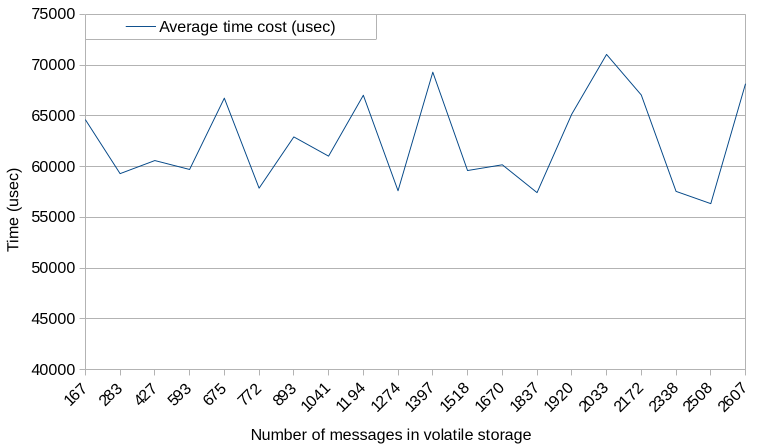
\includegraphics[width=8cm]{rollback_timing_average_new.png}
	\caption{Average rollback cost}
	\label{fig:average_rollback}
\end{figure}\noindent
The figures \ref{fig:rollback_cost}, \ref{fig:average_rollback} above shows the time cost of the rollback procedure. The line in blue shows the time it took from the moment the process received the control message until normal operation was resumed, the red line shows the amount of messages in volatile memory that where stored by the process performing the rollback. This shows that this is a costly procedure since it takes almost 0,1 second most of the time. However at the 1st, 4th, 6th and 10th time the rollback was performed shows a discrepancy, it takes considerably less time to complete the rollback. This is due to that there has not been a checkpoint in between the other process crashing and the process performing the rollback to receive the control message and thus it will not have to remove any checkpoints. The only thing the rollback then does is to replay, resend and remove messages from volatile memory. This indicates that the removal of checkpoints is a costly operation.
\par
\begin{figure}[h]
	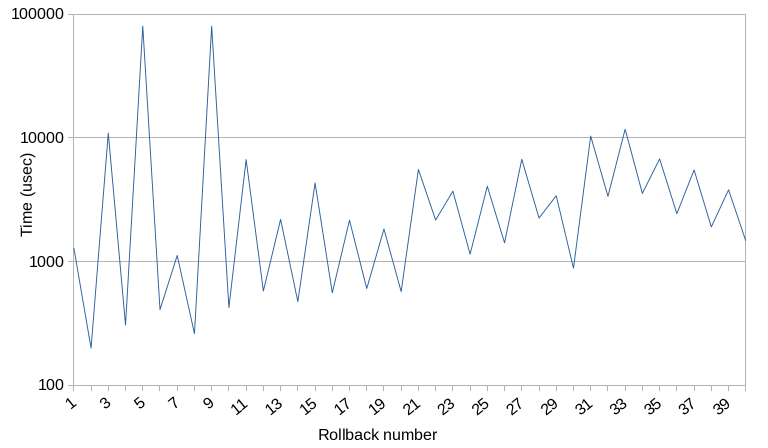
\includegraphics[width=8cm]{concurrent_rollback_cost_new.png}
	\caption{Concurrent rollback cost}
	\label{fig:concurrent_rollback}
\end{figure}\noindent
In figure \ref{fig:concurrent_rollback} the rollback cost when dealing with concurrent failures, all odd  number rollbacks are the from the initial failure the even rollback numbers indicate the concurrent failure after the initial one.
\par This shows that the concurrent failure will cause the rollback to be performed much faster than the rollback performed after the initial failure. This is logical since the rollback procedure has already been performed, only message that needed to be resent will again need to be resent, the other parts of the rollback have already been performed at the rollback caused by the initial failure.


\subsection{Correctness indication}%think of some scenarios to test.



\subsection{Future Work}


\section{Conclusion}
With this we can conclude that the memory overhead does increase proportionate to the number of processes communicating, however we can also conclude that the sending and receiving performance is not greatly affected by the number of processes communicating. The rollback performance as well as the commit receive performance shows that the removing of checkpoints a costly operation. In general is rolling back a costly operation while restarting is a relatively cheap operation.
\newpage
\onecolumn

\appendix

\section{pet-kea.cpp}

\lstinputlisting{code/appendix_pet-kea.cpp}

\section{pet-kea.hpp}

\lstinputlisting{code/appendix_pet-kea.hpp}

\bibliographystyle{IEEEtran}

\bibliography{mybib}

\end{document}
